\documentclass[11pt,a4paper]{article}
\usepackage{fontspec}
\setmainfont{DejaVu Sans}
\setsansfont{DejaVu Sans}
\setmonofont{DejaVu Sans Mono}[Scale=0.82]

\usepackage[a4paper,margin=2.3cm,headheight=14pt]{geometry}
\usepackage{parskip}
\usepackage{enumitem}
\setlist{noitemsep,topsep=3pt,leftmargin=1.4em}
\usepackage{booktabs}
\usepackage{graphicx}
\usepackage{amsmath}

\usepackage{xcolor}
\definecolor{novaNavy}{HTML}{0B2C5C}
\definecolor{novaCyan}{HTML}{0A8FB0}
\definecolor{novaGray}{HTML}{5B7088}
\definecolor{novaInk}{HTML}{1A2433}
\definecolor{ideBg}{HTML}{0E1626}
\definecolor{ideFg}{HTML}{D6E8F0}
\definecolor{ideComment}{HTML}{6A7A8C}
\definecolor{ideFunc}{HTML}{61AFEF}

\usepackage{titlesec}
\titleformat{\section}{\color{novaNavy}\Large\bfseries\sffamily}{\thesection}{0.6em}{}[\vspace{2pt}{\color{novaCyan}\titlerule[1pt]}]
\titleformat{\subsection}{\color{novaNavy}\large\bfseries\sffamily}{\thesubsection}{0.6em}{}
\titleformat{\subsubsection}{\color{novaCyan}\normalsize\bfseries\sffamily}{\thesubsubsection}{0.6em}{}
\titlespacing*{\section}{0pt}{16pt}{8pt}
\titlespacing*{\subsection}{0pt}{11pt}{5pt}
\titlespacing*{\subsubsection}{0pt}{9pt}{3pt}

\usepackage{fancyhdr}
\pagestyle{fancy}
\fancyhf{}
\renewcommand{\headrulewidth}{0pt}
\renewcommand{\footrulewidth}{0.4pt}
\renewcommand{\footrule}{\hbox to\headwidth{\color{novaCyan}\leaders\hrule height \footrulewidth\hfill}}
\fancyfoot[L]{\small\color{novaGray}\sffamily NOVA --- Documentazione}
\fancyfoot[R]{\small\color{novaGray}\sffamily Pagina \thepage}

\usepackage{minted}
\usepackage[most]{tcolorbox}
\newminted[pycode]{python}{fontsize=\footnotesize,breaklines=true,breakanywhere=true,tabsize=4,autogobble,style=monokai,formatcom=\color{ideFg}}
\newminted[bashcode]{bash}{fontsize=\footnotesize,breaklines=true,breakanywhere=true,tabsize=2,autogobble,style=monokai,formatcom=\color{ideFg}}
\newmintinline[pyin]{python}{style=monokai,bgcolor=ideBg}

\newtcolorbox{idebox}{colback=ideBg,colframe=ideBg,boxrule=0pt,arc=3pt,left=8pt,right=8pt,top=4pt,bottom=4pt}

\definecolor{whyBg}{HTML}{E3F4F8}
\newtcolorbox{nota}{colback=whyBg,colframe=novaCyan,boxrule=0pt,leftrule=3pt,arc=1pt,left=8pt,right=8pt,top=6pt,bottom=6pt,fontupper=\small}

\definecolor{warnBg}{HTML}{FAEEDA}
\definecolor{warnBar}{HTML}{B8791A}
\newtcolorbox{attenzione}{colback=warnBg,colframe=warnBar,boxrule=0pt,leftrule=3pt,arc=1pt,left=8pt,right=8pt,top=6pt,bottom=6pt,fontupper=\small}

\usepackage{hyperref}
\hypersetup{colorlinks=true,linkcolor=novaCyan,urlcolor=novaCyan,pdfborder={0 0 0}}

\renewcommand{\arraystretch}{1.25}
\usepackage{colortbl}
\definecolor{tblHead}{HTML}{0B2C5C}
\definecolor{tblAlt}{HTML}{EEF6F9}


\def\oggidata{26 agosto 2026}

\begin{document}
\sffamily

\thispagestyle{empty}
\vspace*{3cm}
\begin{center}
  {\color{novaNavy}\fontsize{40}{44}\selectfont\bfseries NOVA}\\[8pt]
  {\color{novaCyan}\Large Documentazione}\\[12pt]
  {\color{novaGray}\large Gaze-guided Salient Object Ranking}\\[2.2cm]

  {\large\color{novaInk} Riccardo Schiavo \quad$\cdot$\quad Eros Patarini}\\[6pt]
  {\color{novaInk} Industrial Applications of Computer Vision}\\
  {\color{novaInk} Università degli Studi di Padova --- A.A. 2025--26}\\[1.2cm]

  {\color{novaGray}\small \oggidata}
\end{center}

\vfill
\begin{nota}
\textbf{Come è organizzato questo documento.}

\medskip
La \textbf{Parte I} spiega il funzionamento generale: il problema, la pipeline dall'immagine alle
metriche, l'architettura del codice.

\medskip
La \textbf{Parte II} scende nel dettaglio, file per file: per ognuno la funzione che svolge, poi
il codice sezionato riga per riga con il motivo di ogni scelta. I file sono presentati in ordine
di dipendenza, così non si incontra mai un riferimento a qualcosa non ancora spiegato.
\end{nota}
\vspace{0.6cm}

\newpage
\tableofcontents
\newpage

% ===================== PARTE I: PANORAMICA =====================
\part{Come funziona il progetto}

\section{Il problema}

La \textbf{visual saliency prediction} consiste nel predire quali zone di un'immagine attirano
l'attenzione visiva di un osservatore umano. L'output è una \emph{saliency map}: un'immagine in
scala di grigi dove il valore di ogni pixel indica quanta attenzione quel punto riceve.

NOVA confronta più modelli di saliency valutandoli contro una ground truth costruita con
\textbf{click del mouse come proxy del gaze}. Come passo finale, le saliency map vengono
combinate con dei bounding box per produrre un \textbf{ranking degli oggetti} per importanza
visiva.

\begin{nota}
\textbf{Perché i click e non un eye-tracker.} Un eye-tracker è costoso e non disponibile. La
soluzione adottata non è un ripiego improvvisato: è il metodo con cui è stato costruito
\textbf{SALICON}, uno dei dataset di riferimento della letteratura. Chiedendo a una persona di
cliccare sui punti che attirano la sua attenzione si ottiene una distribuzione spaziale
fortemente correlata con quella delle fissazioni oculari reali.
\end{nota}

\subsection{Input e output}

\begin{center}
\begin{tabular}{l p{10.4cm}}
\toprule
\rowcolor{tblHead}\textcolor{white}{\textbf{}} & \textcolor{white}{\textbf{}} \\
\midrule
\textbf{Input} & Una singola immagine RGB \\
\rowcolor{tblAlt} \textbf{Output 1} & Una saliency map per ciascun modello: \pyin{float32}, valori in $[0,1]$, stesse dimensioni dell'immagine \\
\textbf{Output 2} & Una lista di oggetti ordinati per importanza visiva predetta \\
\rowcolor{tblAlt} \textbf{Output 3} & Tabelle di metriche che quantificano l'accordo di ogni modello con la ground truth \\
\bottomrule
\end{tabular}
\end{center}

\section{La pipeline}

\begin{idebox}
\begin{Verbatim}[commandchars=\\\{\},fontsize=\footnotesize]
\textcolor{ideComment}{[1] RACCOLTA}
    \textcolor{ideFg}{foto in prima persona}  ──►  \textcolor{ideFunc}{data/eval/}

\textcolor{ideComment}{[2] ANNOTAZIONE}                                    \textcolor{ideComment}{annotate.py}
    \textcolor{ideFg}{click ordinati (3-6 per immagine, più annotatori)}
                            │
                            ▼
                  \textcolor{ideFunc}{data/annotations/*.json}

\textcolor{ideComment}{[3] GROUND TRUTH}                          \textcolor{ideComment}{ground_truth.py}
    \textcolor{ideFg}{click}  ──┬──►  \textcolor{ideFunc}{mappa di fissazione}   \textcolor{ideComment}{(binaria)}
             └──►  \textcolor{ideFunc}{heatmap continua}      \textcolor{ideComment}{(Gaussiane sommate)}

\textcolor{ideComment}{[4] PREDIZIONE}                              \textcolor{ideComment}{registry.py}
    \textcolor{ideFg}{immagine}  ──►  \textcolor{ideFunc}{Center Prior / Spectral Residual / Itti-Koch}
                            │
                            ▼
                     \textcolor{ideFunc}{saliency map}

\textcolor{ideComment}{[5] CONFRONTO}                                 \textcolor{ideComment}{metrics.py}
    \textcolor{ideFg}{saliency map  vs  ground truth}
                            │
                            ▼
              \textcolor{ideFunc}{CC, SIM, KL, NSS, AUC-Judd}

\textcolor{ideComment}{[6] RANKING}                                   \textcolor{ideComment}{objects.py}
    \textcolor{ideFg}{saliency + box}  ──►  \textcolor{ideFunc}{ranking predetto}
    \textcolor{ideFg}{click + box}     ──►  \textcolor{ideFunc}{ranking di riferimento}
                            │
                            ▼
            \textcolor{ideFunc}{Spearman, Kendall, Top-1}
\end{Verbatim}
\end{idebox}

\subsection{Un esempio concreto}

\begin{center}
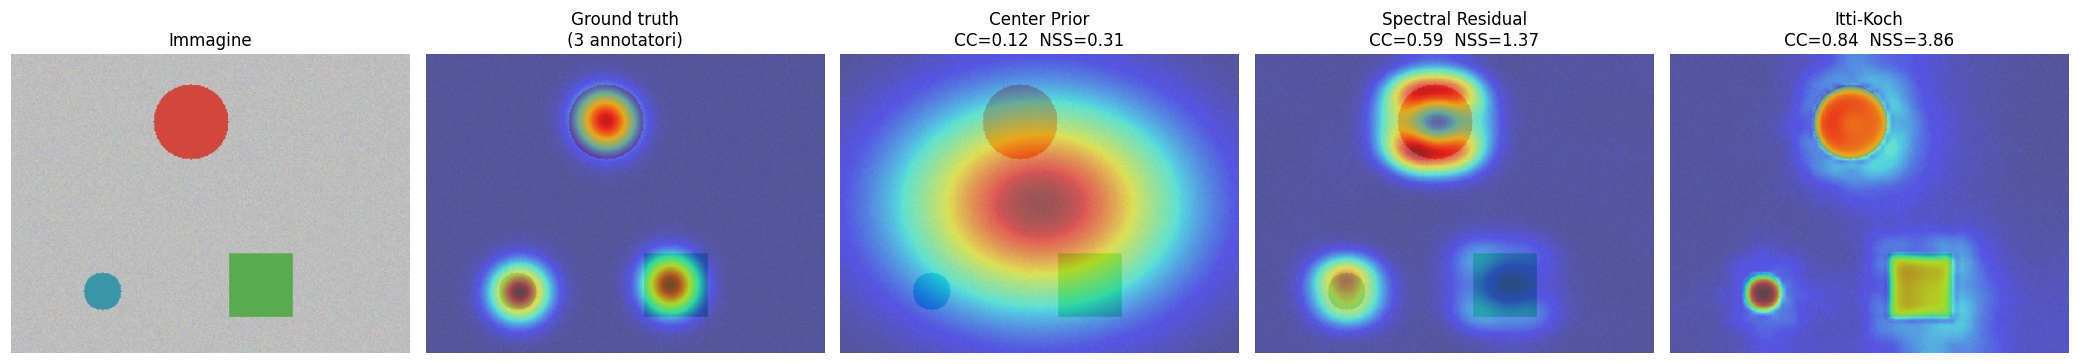
\includegraphics[width=\textwidth]{pipeline_example.png}
\end{center}

Da sinistra: l'immagine, la ground truth costruita dai click di tre annotatori, e le predizioni
dei tre modelli con le rispettive metriche. Si vede il progresso: il center prior illumina il
centro ignorando gli oggetti, Spectral Residual li individua parzialmente, Itti-Koch li coglie
tutti e tre.

\section{L'architettura}

\subsection{I tre livelli}

\begin{center}
\begin{tabular}{l p{8.8cm}}
\toprule
\rowcolor{tblHead}\textcolor{white}{\textbf{Livello}} & \textcolor{white}{\textbf{Responsabilità}} \\
\midrule
\texttt{src/baselines/} & I modelli: immagine $\to$ saliency map \\
\rowcolor{tblAlt} \texttt{src/registry.py} & Uniformare l'accesso ai modelli \\
\texttt{src/visualization.py} & Saliency map $\to$ immagine guardabile \\
\rowcolor{tblAlt} \texttt{app.py}, \texttt{annotate.py} & Solo interfaccia: layout ed eventi \\
\bottomrule
\end{tabular}
\end{center}

\begin{nota}
\textbf{Perché non scrivere tutto in \texttt{app.py}.} Sarebbe più corto e funzionerebbe
identicamente, ma: (1) un'interfaccia grafica non si testa automaticamente, la logica sotto sì;
(2) gli script di valutazione riuserebbero le stesse funzioni, che andrebbero duplicate; (3)
aggiungere un modello richiederebbe di toccare più punti invece di uno solo.
\end{nota}

\subsection{Il contratto della saliency map}

Tutti i modelli rispettano lo stesso contratto di uscita:

\begin{center}
\begin{tabular}{>{\bfseries}l l}
\toprule
\rowcolor{tblHead}\textcolor{white}{\textbf{Proprietà}} & \textcolor{white}{\textbf{Valore}} \\
\midrule
Tipo & \pyin{np.float32} \\
\rowcolor{tblAlt} Range & $[0, 1]$ --- 0 = ignorato, 1 = massima attenzione \\
Dimensioni & identiche a \pyin{(height, width)} dell'input \\
\bottomrule
\end{tabular}
\end{center}

Deciso una volta e valido per tutti. Se ogni modello restituisse un formato diverso servirebbero
conversioni sparse in tutto il codice, con rischio concreto di confronti falsati.

\subsection{La convenzione BGR}

OpenCV carica le immagini in ordine \textbf{BGR}, non RGB. Tutto il progetto adotta questa
convenzione; la conversione a RGB avviene solo al momento di visualizzare.

\begin{attenzione}
\textbf{Errore silenzioso da conoscere.} Passare un'immagine RGB a una funzione che si aspetta
BGR non solleva nessuna eccezione: la forma è giusta e l'immagine resta visualizzabile.
Semplicemente rosso e blu sono scambiati --- e Itti-Koch, che ha canali di opponenza cromatica,
produce risultati sbagliati senza alcun segnale.
\end{attenzione}

\section{Struttura dei file}

\begin{idebox}
\begin{Verbatim}[commandchars=\\\{\},fontsize=\footnotesize]
\textcolor{ideFunc}{app.py}                   \textcolor{ideComment}{interfaccia web di confronto}
\textcolor{ideFunc}{annotate.py}              \textcolor{ideComment}{interfaccia web di annotazione}
\textcolor{ideFunc}{requirements.txt}
\textcolor{ideFunc}{src/}
├── \textcolor{ideFg}{registry.py}          \textcolor{ideComment}{registro centrale dei modelli}
├── \textcolor{ideFg}{visualization.py}     \textcolor{ideComment}{heatmap, overlay, marcatori}
├── \textcolor{ideFunc}{baselines/}
│   ├── \textcolor{ideFg}{center_prior.py}       \textcolor{ideComment}{baseline: Gaussiana centrata}
│   ├── \textcolor{ideFg}{spectral_residual.py}  \textcolor{ideComment}{FFT + residuo spettrale}
│   └── \textcolor{ideFg}{itti_koch.py}          \textcolor{ideComment}{center-surround multi-scala}
├── \textcolor{ideFunc}{annotation/}
│   ├── \textcolor{ideFg}{store.py}              \textcolor{ideComment}{persistenza delle annotazioni}
│   └── \textcolor{ideFg}{ground_truth.py}       \textcolor{ideComment}{click -> heatmap e fissazioni}
├── \textcolor{ideFunc}{evaluation/}
│   └── \textcolor{ideFg}{metrics.py}            \textcolor{ideComment}{tutte le metriche}
└── \textcolor{ideFunc}{ranking/}
    └── \textcolor{ideFg}{objects.py}            \textcolor{ideComment}{ranking degli oggetti}
\textcolor{ideFunc}{scripts/run_evaluation.py} \textcolor{ideComment}{valutazione -> tabelle CSV}
\textcolor{ideFunc}{tests/test_all.py}         \textcolor{ideComment}{56 controlli}
\end{Verbatim}
\end{idebox}

\subsection{Comandi}

\begin{idebox}
\begin{bashcode}
python3 -m venv venv
source venv/bin/activate          # Windows: venv\Scripts\activate
pip install -r requirements.txt

python app.py                     # interfaccia di confronto
python annotate.py --images data/eval   # interfaccia di annotazione
python scripts/run_evaluation.py  # valutazione completa
python tests/test_all.py          # 56 test
\end{bashcode}
\end{idebox}

\newpage

% ===================== PARTE II: FILE PER FILE =====================
\part{Il codice, file per file}

I file sono presentati in \textbf{ordine di dipendenza}: prima quelli che non dipendono da
nessuno, poi quelli che li usano. Leggendoli in quest'ordine non si incontra mai un riferimento
a qualcosa non ancora spiegato.

\section{\texttt{src/baselines/center\_prior.py}}

Il modello più semplice del progetto, e il punto migliore da cui iniziare a leggere il codice.

\subsection{A cosa serve}

Genera una Gaussiana 2D fissa al centro dell'immagine, \textbf{ignorando completamente il
contenuto}. A parità di dimensioni restituisce sempre la stessa identica mappa.

\begin{nota}
\textbf{Perché una baseline così banale è indispensabile.} Nella letteratura sull'attenzione
visiva è documentato il \emph{center bias}: le persone guardano il centro di una scena molto più
spesso della periferia, sia perché chi scatta tende a inquadrare al centro il soggetto, sia per
una tendenza oculomotoria naturale.

\medskip
Un modello che non batte questa Gaussiana non sta estraendo \emph{nessuna} informazione
dall'immagine: sta solo riscoprendo il center bias. Le linee guida del corso richiedono
esplicitamente almeno una baseline, e questa è la scelta standard per la saliency.
\end{nota}

\subsection{La firma}

\begin{idebox}
\begin{pycode}
def center_prior_saliency(image_shape, sigma_frac=0.25):
\end{pycode}
\end{idebox}

\begin{center}
\begin{tabular}{>{\ttfamily}l l p{6.9cm}}
\toprule
\rowcolor{tblHead}\textcolor{white}{\textbf{Parametro}} & \textcolor{white}{\textbf{Tipo}} & \textcolor{white}{\textbf{Significato}} \\
\midrule
image\_shape & tuple(int,int) & \pyin{(altezza, larghezza)}. Si passa la \emph{forma}, non l'immagine. \\
\rowcolor{tblAlt} sigma\_frac & float & Deviazione standard come frazione delle dimensioni. \\
\bottomrule
\end{tabular}
\end{center}

\begin{nota}
\textbf{Perché la firma accetta la forma e non l'immagine.} È una scelta deliberata di
\emph{design comunicativo}: la firma stessa dichiara che il modello non guarda mai il contenuto.
Accettare l'immagine e poi ignorarla sarebbe funzionalmente identico ma fuorviante per chi legge
il codice.
\end{nota}

\subsection{Il corpo, riga per riga}

\subsubsection{Centro e deviazioni standard}

\begin{idebox}
\begin{pycode}
height, width = image_shape

cx = width / 2.0
cy = height / 2.0
sigma_x = sigma_frac * width
sigma_y = sigma_frac * height
\end{pycode}
\end{idebox}

\pyin{cx} e \pyin{cy} sono le coordinate del centro geometrico. La divisione è per \pyin{2.0}
(float) e non per \pyin{2} (int) per evitare la divisione intera su immagini di dimensione
dispari.

\pyin{sigma_x} e \pyin{sigma_y} sono \textbf{separati e proporzionali} alle rispettive
dimensioni. Con un unico $\sigma$ espresso in pixel:

\begin{itemize}
  \item su un'immagine 320$\times$240 la macchia coprirebbe una frazione diversa della larghezza
  rispetto all'altezza --- un'ellisse schiacciata rispetto alla forma dell'immagine;
  \item la stessa scena a risoluzione 4K avrebbe una macchia relativamente minuscola.
\end{itemize}

\subsubsection{La griglia di coordinate}

\begin{idebox}
\begin{pycode}
x = np.arange(width, dtype=np.float32)
y = np.arange(height, dtype=np.float32)
xx, yy = np.meshgrid(x, y)
\end{pycode}
\end{idebox}

\pyin{np.arange(width)} produce il vettore $[0, 1, 2, \ldots, \text{width}-1]$.
\pyin{np.meshgrid} li combina in due matrici delle dimensioni dell'immagine:

\begin{itemize}
  \item \pyin{xx[i, j] == j} --- la coordinata orizzontale (colonna) di ogni pixel;
  \item \pyin{yy[i, j] == i} --- la coordinata verticale (riga) di ogni pixel.
\end{itemize}

Avendo le coordinate come matrici, la Gaussiana si calcola su tutti i pixel in \emph{una sola}
operazione vettorizzata, senza cicli \pyin{for} annidati --- che in Python sarebbero ordini di
grandezza più lenti.

\begin{attenzione}
\textbf{Trappola di indicizzazione.} In numpy il primo indice è la \emph{riga} ($y$), il secondo
la \emph{colonna} ($x$): si scrive \pyin{img[y, x]}. È l'inverso della notazione matematica
$(x, y)$. Praticamente tutti gli scambi $x$/$y$ in questo progetto nascono da qui.
\end{attenzione}

\subsubsection{La Gaussiana}

\begin{idebox}
\begin{pycode}
exponent = -((xx - cx) ** 2 / (2.0 * sigma_x ** 2)
             + (yy - cy) ** 2 / (2.0 * sigma_y ** 2))
gauss = np.exp(exponent)
\end{pycode}
\end{idebox}

Implementazione diretta della Gaussiana 2D separabile:
\[
G(x,y) = \exp\!\left(-\left[\frac{(x-c_x)^2}{2\sigma_x^2} + \frac{(y-c_y)^2}{2\sigma_y^2}\right]\right)
\]

L'esponente è calcolato separatamente per leggibilità. Il valore massimo è $1.0$, raggiunto
esattamente al centro dove entrambi i termini si annullano.

\subsubsection{La normalizzazione}

\begin{idebox}
\begin{pycode}
def _normalize(saliency_map):
    minimum, maximum = saliency_map.min(), saliency_map.max()
    if maximum - minimum > 0:
        saliency_map = (saliency_map - minimum) / (maximum - minimum)
    else:
        saliency_map = np.zeros_like(saliency_map)
    return saliency_map.astype(np.float32)
\end{pycode}
\end{idebox}

Normalizzazione \emph{min-max}: sottrae il minimo e divide per l'escursione, portando i valori
in $[0,1]$.

\begin{nota}
\textbf{Perché normalizzare se il massimo è già 1.0.} Tre motivi: (1) il minimo non è
necessariamente 0, quindi il range va comunque riscalato; (2) rende il contratto identico a
quello degli altri modelli, dove la normalizzazione è indispensabile; (3) il ramo \pyin{else}
protegge dal caso degenere di mappa costante --- qui non può accadere, ma negli altri modelli sì,
e avere lo stesso schema ovunque riduce il rischio di dimenticarlo dove serve.
\end{nota}

Il prefisso \pyin{_} nel nome segnala che è una funzione interna al modulo, non parte
dell'interfaccia pubblica.

\section{\texttt{src/baselines/spectral\_residual.py}}

Riferimento: Hou \& Zhang, \emph{Saliency Detection: A Spectral Residual Approach}, CVPR 2007.

\subsection{L'idea}

Le immagini naturali, mediamente, hanno uno spettro di ampiezza molto regolare: le basse
frequenze dominano e l'energia decade in modo prevedibile al crescere della frequenza. Questa
regolarità è la parte \textbf{ridondante} di una scena --- ciò che tutte le immagini hanno in
comune.

L'ipotesi del metodo: \emph{ciò che devia dall'andamento atteso è l'informazione interessante}.
Si stima l'andamento atteso sfocando il logaritmo dello spettro, lo si sottrae, e ciò che resta
--- il \textbf{residuo spettrale} --- indica le frequenze statisticamente anomale.

\begin{nota}
\textbf{Perché funziona pur essendo ``solo'' un trucco statistico.} Un oggetto saliente ha
tipicamente bordi netti, una texture diversa dallo sfondo, una forma compatta: tutte
caratteristiche che producono energia a frequenze non generiche rispetto al resto della scena.
Il metodo non capisce cosa sia un oggetto, ma la statistica è un buon sostituto --- e costa circa
trenta righe di codice, senza alcun addestramento.
\end{nota}

\subsection{La pipeline in sette passi}

\subsubsection{Passo 1 --- Scala di grigi}

\begin{idebox}
\begin{pycode}
original_h, original_w = image.shape[:2]

if image.ndim == 3 and image.shape[2] == 3:
    gray = cv2.cvtColor(image, cv2.COLOR_BGR2GRAY)
else:
    gray = image.copy()
\end{pycode}
\end{idebox}

Le dimensioni originali si salvano \emph{subito}: serviranno alla fine per riportare la mappa
alla risoluzione di partenza.

Il controllo \pyin{image.ndim == 3 and image.shape[2] == 3} rende la funzione tollerante: accetta
sia immagini a colori sia già in scala di grigi. Il \pyin{.copy()} nel ramo \pyin{else} evita di
lavorare sullo stesso array passato dal chiamante.

\begin{attenzione}
Questo passo è la causa del limite più importante del metodo: \textbf{l'informazione cromatica
viene distrutta}. Un oggetto che si distingue solo per tinta ma non per luminosità diventa
invisibile al modello. Il fenomeno è verificato numericamente nella sezione dei test.
\end{attenzione}

\subsubsection{Passo 2 --- Riduzione di risoluzione}

\begin{idebox}
\begin{pycode}
small = cv2.resize(gray, target_size,
                   interpolation=cv2.INTER_AREA).astype(np.float32)
\end{pycode}
\end{idebox}

Il default \pyin{target_size=(64, 64)} è il valore del paper originale. La saliency è un fenomeno
a bassa frequenza spaziale --- interessa \emph{dove} guardare, non i dettagli fini --- quindi
lavorare a piena risoluzione non aggiunge informazione e costa molto di più.

\pyin{INTER_AREA} è l'interpolazione corretta per \emph{rimpicciolire}: calcola la media dei
pixel dell'area sorgente che confluisce in ogni pixel destinazione. Le alternative
(\pyin{INTER_LINEAR}, \pyin{INTER_NEAREST}) campionano pochi pixel e producono
\emph{aliasing} --- artefatti ad alta frequenza che qui sarebbero disastrosi, dato che il metodo
analizza proprio lo spettro delle frequenze.

Il cast a \pyin{float32} è necessario prima della FFT: su \pyin{uint8} i calcoli andrebbero in
overflow.

\subsubsection{Passo 3 --- FFT e separazione ampiezza/fase}

\begin{idebox}
\begin{pycode}
spectrum = np.fft.fft2(small)
amplitude = np.abs(spectrum)
phase = np.angle(spectrum)
\end{pycode}
\end{idebox}

\pyin{np.fft.fft2} produce una matrice di numeri \emph{complessi}. Ogni numero complesso
$z = a + bi$ si può leggere in forma polare come $z = |z| e^{i\theta}$:

\begin{itemize}
  \item \pyin{np.abs(spectrum)} $= |z|$ --- l'\textbf{ampiezza}: \emph{quanta} energia c'è a
  quella frequenza;
  \item \pyin{np.angle(spectrum)} $= \theta$ --- la \textbf{fase}: \emph{dove} sono posizionate
  le strutture nell'immagine.
\end{itemize}

\subsubsection{Passo 4 --- Il residuo}

\begin{idebox}
\begin{pycode}
log_amplitude = np.log(amplitude + 1e-8)
avg_log_amplitude = cv2.blur(log_amplitude, (3, 3))
spectral_residual = log_amplitude - avg_log_amplitude
\end{pycode}
\end{idebox}

Tre righe, tre decisioni:

\begin{description}[leftmargin=1.2em,style=nextline]
\item[\pyin{np.log(...)}] L'ampiezza varia di diversi ordini di grandezza tra basse e alte
frequenze. Il logaritmo comprime questo range, rendendo l'andamento generale approssimabile con
una semplice media locale.

\item[\pyin{+ 1e-8}] Protezione da $\log(0)$, che darebbe $-\infty$ e propagherebbe NaN in tutto
il calcolo. Il valore è abbastanza piccolo da non alterare i risultati.

\item[\pyin{cv2.blur(..., (3,3))}] Filtro a media mobile: stima l'andamento ``atteso'' dello
spettro. La differenza tra spettro reale e atteso è il \textbf{residuo}, cioè la parte
statisticamente anomala.
\end{description}

\subsubsection{Passo 5 --- Ricostruzione}

\begin{idebox}
\begin{pycode}
reconstructed = np.fft.ifft2(np.exp(spectral_residual + 1j * phase))
saliency = (np.abs(reconstructed) ** 2).astype(np.float32)
\end{pycode}
\end{idebox}

Riga densa, va letta dall'interno verso l'esterno:

\begin{enumerate}
  \item \pyin{spectral_residual + 1j * phase} --- ricompone un numero complesso usando il residuo
  come parte reale (siamo nel dominio logaritmico) e la fase \textbf{originale} come parte
  immaginaria. \pyin{1j} è l'unità immaginaria in Python.
  \item \pyin{np.exp(...)} --- annulla il logaritmo del passo 4, tornando al dominio lineare.
  \item \pyin{np.fft.ifft2(...)} --- FFT inversa: dal dominio delle frequenze allo spazio
  immagine.
  \item \pyin{np.abs(...) ** 2} --- modulo al quadrato, cioè l'\emph{energia}. Sempre positiva,
  come deve essere una saliency map.
\end{enumerate}

\begin{nota}
\textbf{Perché si conserva la fase originale.} Il metodo modifica solo l'ampiezza. Se si
scartasse la fase e se ne usasse una casuale, la ricostruzione non avrebbe alcuna relazione
spaziale con la scena: si otterrebbe rumore. La fase è ciò che àncora l'informazione alla
posizione.
\end{nota}

\subsubsection{Passo 6 --- Smoothing}

\begin{idebox}
\begin{pycode}
ksize = int(np.ceil(sigma * 6)) | 1
saliency = cv2.GaussianBlur(saliency, (ksize, ksize), sigma)
\end{pycode}
\end{idebox}

\pyin{cv2.GaussianBlur} richiede una dimensione di kernel \emph{dispari}.

\begin{description}[leftmargin=1.2em,style=nextline]
\item[\pyin{sigma * 6}] Regola pratica: una Gaussiana è praticamente nulla oltre $\pm 3\sigma$,
quindi un kernel di $6\sigma$ la contiene quasi interamente.
\item[\pyin{| 1}] OR bit-a-bit con 1: forza a 1 il bit meno significativo, trasformando qualsiasi
numero pari nel dispari successivo ($12 \to 13$, $13 \to 13$). Idioma compatto per ``arrotonda al
dispari''.
\end{description}

Lo smoothing non è cosmetico: la ricostruzione grezza è molto puntinata, mentre l'attenzione
umana si concentra su \emph{regioni}, non su singoli pixel isolati.

\subsubsection{Passo 7 --- Ritorno alla risoluzione originale}

\begin{idebox}
\begin{pycode}
saliency = _normalize(saliency)
return cv2.resize(saliency, (original_w, original_h),
                  interpolation=cv2.INTER_LINEAR)
\end{pycode}
\end{idebox}

Qui si usa \pyin{INTER_LINEAR} perché si sta \emph{ingrandendo}, il caso opposto al passo 2.

\begin{attenzione}
\pyin{cv2.resize} vuole la dimensione come \pyin{(width, height)}, mentre \pyin{shape} di numpy è
\pyin{(height, width)}. L'ordine invertito è una fonte classica di bug silenziosi: l'immagine
esce distorta senza alcun errore.
\end{attenzione}

\section{\texttt{src/baselines/itti\_koch.py}}

Riferimento: Itti, Koch \& Niebur, \emph{A Model of Saliency-Based Visual Attention for Rapid
Scene Analysis}, IEEE TPAMI 1998. Il file più articolato del progetto: una funzione pubblica e
quattro funzioni di supporto.

\subsection{L'idea}

\textbf{Un punto è saliente se spicca rispetto a ciò che lo circonda.} Il modello non riconosce
oggetti: misura contrasto locale su tre canali che il sistema visivo umano elabora in parallelo
nelle prime fasi della visione.

\begin{center}
\begin{tabular}{l p{9.4cm}}
\toprule
\rowcolor{tblHead}\textcolor{white}{\textbf{Canale}} & \textcolor{white}{\textbf{Corrispettivo biologico}} \\
\midrule
Intensità & Contrasto di luminanza, la via più antica ed elementare. \\
\rowcolor{tblAlt} Colore & Opponenza rosso/verde e blu/giallo: è il modo in cui la retina codifica
effettivamente il colore, tramite cellule gangliari antagoniste. \\
Orientazione & Filtri di Gabor a 0°, 45°, 90°, 135°: modello classico delle cellule semplici
della corteccia visiva primaria (V1). \\
\bottomrule
\end{tabular}
\end{center}

\subsection{Le funzioni di supporto}

\subsubsection{\texttt{\_gaussian\_pyramid}}

\begin{idebox}
\begin{pycode}
def _gaussian_pyramid(channel, levels):
    pyramid = [channel.astype(np.float32)]
    for _ in range(levels - 1):
        pyramid.append(cv2.pyrDown(pyramid[-1]).astype(np.float32))
    return pyramid
\end{pycode}
\end{idebox}

Restituisce una \emph{lista} di array: \pyin{pyramid[0]} è l'immagine originale,
\pyin{pyramid[1]} è a metà risoluzione, \pyin{pyramid[2]} a un quarto, e così via.

Ogni livello si costruisce da \pyin{pyramid[-1]}, cioè dall'ultimo aggiunto: la riduzione è
cumulativa.

\begin{nota}
\textbf{A cosa serve la piramide.} Permette di guardare la scena ``a più distanze'': un dettaglio
fine e un oggetto grande producono contrasto a scale diverse, e senza la piramide se ne
coglierebbe solo una.

\medskip
\pyin{cv2.pyrDown} non si limita a scartare pixel: applica prima una sfocatura Gaussiana e poi
sottocampiona. Senza la sfocatura si avrebbe aliasing.
\end{nota}

\subsubsection{\texttt{\_resize\_to}}

\begin{idebox}
\begin{pycode}
def _resize_to(feature_map, shape):
    return cv2.resize(feature_map, (shape[1], shape[0]),
                      interpolation=cv2.INTER_LINEAR)
\end{pycode}
\end{idebox}

Wrapper minimale che esiste per un solo motivo: \textbf{isolare in un punto unico} l'inversione
\pyin{(height, width)} $\to$ \pyin{(width, height)}. Lo scambio \pyin{shape[1], shape[0]} compare
così una volta sola nel modulo, invece che in ogni punto in cui serve un resize.

\subsubsection{\texttt{\_center\_surround}}

\begin{idebox}
\begin{pycode}
def _center_surround(pyramid, center_scales=(2, 3), deltas=(3, 4)):
    maps = []
    for c in center_scales:
        for delta in deltas:
            s = c + delta
            if s >= len(pyramid):
                continue
            center = pyramid[c]
            surround = _resize_to(pyramid[s], center.shape[:2])
            maps.append(np.abs(center - surround))
    return maps
\end{pycode}
\end{idebox}

Doppio ciclo su $c \in \{2,3\}$ (scala \emph{center}, il dettaglio) e $\delta \in \{3,4\}$, con
$s = c + \delta$ (scala \emph{surround}, il contesto). Le quattro combinazioni sono
$(2,5), (2,6), (3,6), (3,7)$.

Il \pyin{continue} salta le combinazioni in cui $s$ eccede i livelli disponibili: con
\pyin{pyramid_levels=7} (indici $0$--$6$) la coppia $(3,7)$ viene scartata, restano tre mappe per
canale.

Prima della sottrazione, la scala grossolana viene riportata alla risoluzione di quella fine:
sono array di dimensioni diverse e non si potrebbero sottrarre direttamente. Il valore assoluto
serve perché conta l'\emph{entità} del contrasto, non il suo segno --- chiaro su scuro e scuro su
chiaro sono entrambi salienti.

È l'analogo computazionale dei campi recettivi center-surround dei neuroni retinici.

\subsubsection{\texttt{\_normalize\_map} --- l'operatore \texorpdfstring{$N(\cdot)$}{N()}}

La funzione concettualmente più densa del progetto.

\begin{idebox}
\begin{pycode}
def _normalize_map(feature_map, M=10.0):
    feature_map = feature_map - feature_map.min()
    if feature_map.max() > 0:
        feature_map = feature_map / feature_map.max() * M

    local_max = cv2.dilate(feature_map, np.ones((7, 7), np.uint8))
    is_local_max = (feature_map == local_max) & (feature_map < M - 1e-3)
    peaks = feature_map[is_local_max]
    mean_peak = peaks.mean() if peaks.size > 0 else 0.0

    return feature_map * (M - mean_peak) ** 2
\end{pycode}
\end{idebox}

\paragraph{Righe 1--3: portare la mappa in $[0, M]$.}
Scala lineare in un intervallo noto, con $M = 10$ (valore del paper). La scelta esatta è
arbitraria: conta il \emph{rapporto} fra $M$ e la media dei picchi.

\paragraph{Riga 5: trovare i massimi locali con una dilatazione.}
\pyin{cv2.dilate} sostituisce ogni pixel con il massimo della sua vicinanza $7\times7$. Di
conseguenza, un pixel che dopo la dilatazione \emph{vale ancora quanto prima} è esattamente un
massimo locale. È un trucco elegante: identifica tutti i massimi locali con una singola
operazione morfologica invece che con una scansione esplicita.

\paragraph{Riga 6: escludere il massimo globale.}
La condizione \pyin{feature_map < M - 1e-3} scarta il picco più alto, che vale esattamente $M$
dopo la normalizzazione. Interessa la media degli \emph{altri} picchi: è quella che dice se la
mappa ha un vincitore netto o tanti competitori.

\paragraph{Righe 7--8: la media dei picchi, con guardia.}
\pyin{peaks.size > 0} protegge dal caso in cui non ci siano massimi locali oltre al globale:
\pyin{.mean()} su un array vuoto restituirebbe NaN con un warning.

\paragraph{Riga 10: il fattore di enfasi.}
\[
N(\text{mappa}) = \text{mappa} \times (M - \bar{m})^2
\]
dove $\bar{m}$ è la media dei massimi locali.

\begin{center}
\begin{tabular}{l l l}
\toprule
\rowcolor{tblHead}\textcolor{white}{\textbf{Situazione}} & \textcolor{white}{$\bar{m}$} & \textcolor{white}{\textbf{Effetto}} \\
\midrule
Un solo picco netto & bassa & $(M-\bar m)^2$ grande $\to$ mappa \textbf{amplificata} \\
\rowcolor{tblAlt} Molti picchi simili & alta & $(M-\bar m)^2$ piccolo $\to$ mappa \textbf{soppressa} \\
\bottomrule
\end{tabular}
\end{center}

\begin{nota}
\textbf{Perché conta.} Due mappe possono avere lo stesso valore massimo ma significato opposto:
una con un picco isolato indica un elemento davvero distintivo, una con venti picchi di altezza
simile indica rumore diffuso.

\medskip
Senza $N(\cdot)$ un canale rumoroso dominerebbe la somma finale per pura forza bruta. È il
meccanismo che rende il modello \emph{selettivo} invece che additivo --- ed è anche la parte del
paper originale che viene più spesso semplificata nelle reimplementazioni, inclusa la nostra.
\end{nota}

\subsection{La funzione principale}

\subsubsection{Estrazione dei canali}

\begin{idebox}
\begin{pycode}
img = image.astype(np.float32)
b, g, r = cv2.split(img)

intensity = (r + g + b) / 3.0

eps = 1e-3
rg = (r - g) / (intensity + eps)
by = (b - np.minimum(r, g)) / (intensity + eps)
\end{pycode}
\end{idebox}

\pyin{cv2.split} separa i tre canali. L'ordine di destrutturazione è \pyin{b, g, r} perché
OpenCV usa BGR.

Le formule di opponenza cromatica riproducono il modo in cui la retina umana codifica il colore:
non come tre canali indipendenti, ma come \emph{differenze} tra coppie antagoniste. Il giallo è
approssimato da \pyin{np.minimum(r, g)}, dato che percettivamente è la componente comune a rosso
e verde.

\begin{nota}
\textbf{Perché dividere per l'intensità.} Normalizza rispetto alla luminosità: un rosso acceso in
ombra e lo stesso rosso in piena luce hanno valori RGB molto diversi ma la stessa \emph{tinta}.
Dividendo per \pyin{intensity} il canale misura la tinta indipendentemente dall'illuminazione.

\medskip
\pyin{eps = 1e-3} evita la divisione per zero nelle zone quasi nere, dove il colore è comunque
privo di significato percettivo.
\end{nota}

\subsubsection{Filtri di Gabor}

\begin{idebox}
\begin{pycode}
orientation_pyramids = []
for theta_deg in (0, 45, 90, 135):
    kernel = cv2.getGaborKernel(
        ksize=(15, 15), sigma=4.0, theta=np.radians(theta_deg),
        lambd=10.0, gamma=0.5, psi=0,
    )
    orientation_pyramids.append(
        [cv2.filter2D(level, cv2.CV_32F, kernel) for level in intensity_pyr]
    )
\end{pycode}
\end{idebox}

Un filtro di Gabor è una sinusoide modulata da una Gaussiana: risponde fortemente ai bordi che
hanno l'orientamento e la frequenza spaziale a cui è sintonizzato.

\begin{center}
\begin{tabular}{>{\ttfamily}l l p{6.6cm}}
\toprule
\rowcolor{tblHead}\textcolor{white}{\textbf{Parametro}} & \textcolor{white}{\textbf{Valore}} & \textcolor{white}{\textbf{Significato}} \\
\midrule
ksize & (15,15) & Dimensione del kernel: deve contenere almeno un periodo della sinusoide. \\
\rowcolor{tblAlt} sigma & 4.0 & Ampiezza dell'inviluppo Gaussiano: quanto è esteso il filtro. \\
theta & 0--135° & Orientamento a cui è sensibile. \pyin{np.radians} converte: OpenCV vuole radianti. \\
\rowcolor{tblAlt} lambd & 10.0 & Lunghezza d'onda della sinusoide: la ``spaziatura'' dei bordi cercati. \\
gamma & 0.5 & Rapporto d'aspetto: allunga il filtro, rendendolo più selettivo sull'orientamento. \\
\rowcolor{tblAlt} psi & 0 & Sfasamento. A 0 il filtro è simmetrico. \\
\bottomrule
\end{tabular}
\end{center}

Il filtro si applica a \emph{tutti} i livelli della piramide di intensità: da qui la list
comprehension interna. Il risultato sono 4 piramidi, una per orientamento.

\pyin{cv2.CV_32F} forza l'output in float: la risposta di Gabor può essere negativa e su
\pyin{uint8} verrebbe troncata.

\subsubsection{Conspicuity map e combinazione finale}

\begin{idebox}
\begin{pycode}
target_shape = intensity_maps[0].shape

def combine(maps):
    resized = [_resize_to(m, target_shape) for m in maps]
    return _normalize_map(np.sum(resized, axis=0))

conspicuity_intensity = combine(intensity_maps)
conspicuity_color = combine(color_maps)
conspicuity_orientation = combine(orientation_maps)

saliency = (conspicuity_intensity
            + conspicuity_color
            + conspicuity_orientation) / 3.0
\end{pycode}
\end{idebox}

Le mappe center-surround provengono da scale diverse e hanno quindi \emph{dimensioni diverse}:
\pyin{combine} le riporta tutte a una risoluzione comune prima di sommarle.
\pyin{np.sum(resized, axis=0)} somma lungo l'asse della lista, cioè elemento per elemento.

Notare la \textbf{doppia normalizzazione}: prima su ogni singola mappa center-surround, poi di
nuovo sulla somma. Serve perché il confronto avviene a due livelli --- prima tra le scale dello
stesso canale, poi tra i tre canali.

La media finale è \emph{non pesata}: i pesi ottimali sarebbero un parametro da apprendere, e il
modello originale è deliberatamente privo di apprendimento.

\subsection{Semplificazioni dichiarate}

Rispetto al paper originale:

\begin{enumerate}
  \item Coppie di scale center-surround fisse ($c \in \{2,3\}$, $\delta \in \{3,4\}$) invece di
  un set più ampio.
  \item Operatore $N(\cdot)$ a singolo passaggio invece che iterativo.
\end{enumerate}

Entrambe riducono il costo computazionale mantenendo il comportamento qualitativo.
\textbf{Vanno dichiarate nel README}: una semplificazione documentata è una scelta di progetto,
una non documentata è un errore.

\section{\texttt{src/annotation/store.py}}

Gestisce la lettura e la scrittura delle annotazioni.

\subsection{Il protocollo}

L'annotatore guarda un'immagine e clicca \textbf{in ordine di importanza decrescente}. Minimo 3
click, massimo 6.

\begin{idebox}
\begin{pycode}
MIN_CLICKS = 3   # sotto, non esiste un ranking sensato
MAX_CLICKS = 6   # sopra, si cercano cose da cliccare invece di notarle
\end{pycode}
\end{idebox}

\begin{nota}
\textbf{Un compito, due ground truth.} L'ordine dei click non è un dettaglio accessorio: rende lo
stesso gesto utile per due scopi.
\begin{itemize}
  \item i click come \emph{punti di fissazione} $\to$ metriche NSS, AUC-Judd;
  \item l'ordine come \emph{ranking} di importanza $\to$ Spearman, Kendall, Top-1.
\end{itemize}
Un secondo giro di annotazione per il ranking raddoppierebbe il lavoro degli annotatori, che è la
risorsa più scarsa.
\end{nota}

\subsection{Il formato su disco}

Un file JSON \textbf{per annotatore}, non un file unico:

\begin{idebox}
\begin{Verbatim}[commandchars=\\\{\},fontsize=\footnotesize]
\textcolor{ideFg}{data/annotations/riccardo.json}

\textcolor{ideFg}{\{}
  \textcolor{ideFunc}{"annotator"}\textcolor{ideFg}{: "riccardo",}
  \textcolor{ideFunc}{"created_at"}\textcolor{ideFg}{: "2026-08-26T18:00:00+00:00",}
  \textcolor{ideFunc}{"annotations"}\textcolor{ideFg}{: \{}
    \textcolor{ideFunc}{"img_001.jpg"}\textcolor{ideFg}{: \{}
      \textcolor{ideFunc}{"image_size"}\textcolor{ideFg}{: [480, 640],}
      \textcolor{ideFunc}{"clicks"}\textcolor{ideFg}{: [\{"x": 412, "y": 230, "order": 1\}, ...]}
    \textcolor{ideFg}{\}}
  \textcolor{ideFg}{\}}
\textcolor{ideFg}{\}}
\end{Verbatim}
\end{idebox}

\begin{nota}
\textbf{Perché un file per annotatore.} Più persone possono annotare in parallelo senza conflitti
di scrittura, ed escludere un annotatore a posteriori diventa banale (si cancella il suo file).
Un file unico richiederebbe un meccanismo di lock, o produrrebbe sovrascritture silenziose.

\medskip
\textbf{Perché salvare \texttt{image\_size}.} Senza le dimensioni, le coordinate sono prive di
significato: se l'immagine venisse ridimensionata o sostituita, i click punterebbero altrove
senza che nulla lo segnali.
\end{nota}

\subsection{\texttt{\_\_init\_\_} --- normalizzazione del nome}

\begin{idebox}
\begin{pycode}
if not annotator or not annotator.strip():
    raise ValueError("Il nome dell'annotatore non puo' essere vuoto.")

self.annotator = annotator.strip().lower().replace(" ", "_")
self.annotations_dir = annotations_dir
self.path = os.path.join(annotations_dir, f"{self.annotator}.json")
self._data = self._load()
\end{pycode}
\end{idebox}

La catena \pyin{strip().lower().replace(" ", "_")} evita che ``Riccardo'', ``riccardo'' e
``Riccardo~'' diventino tre annotatori distinti --- errore facile quando si digita il nome a
inizio sessione.

\subsection{\texttt{\_save} --- scrittura atomica}

\begin{idebox}
\begin{pycode}
def _save(self):
    os.makedirs(self.annotations_dir, exist_ok=True)
    tmp_path = self.path + ".tmp"
    with open(tmp_path, "w", encoding="utf-8") as f:
        json.dump(self._data, f, indent=2, ensure_ascii=False)
    os.replace(tmp_path, self.path)
\end{pycode}
\end{idebox}

Si scrive su un file temporaneo e poi lo si rinomina.

\begin{attenzione}
\textbf{Perché non scrivere direttamente sul file finale.} Se il processo venisse interrotto a
metà scrittura (crash, chiusura del terminale), il file resterebbe troncato --- JSON non valido,
\emph{tutte} le annotazioni precedenti perse.

\medskip
\pyin{os.replace} è \textbf{atomico} sulla maggior parte dei filesystem: o il file nuovo
sostituisce il vecchio per intero, o non succede nulla. Con sessioni da decine di minuti, questa
protezione non è teorica.
\end{attenzione}

\pyin{ensure_ascii=False} preserva gli accenti nei nomi invece di trasformarli in sequenze di
escape.

\subsection{\texttt{save\_annotation}}

\begin{idebox}
\begin{pycode}
if not MIN_CLICKS <= len(clicks) <= MAX_CLICKS:
    raise ValueError(
        f"Servono da {MIN_CLICKS} a {MAX_CLICKS} click, ricevuti {len(clicks)}."
    )
self._data["annotations"][image_name] = {
    "image_size": list(image_size),
    "clicks": [
        {"x": int(x), "y": int(y), "order": i + 1}
        for i, (x, y) in enumerate(clicks)
    ],
    "annotated_at": datetime.now(timezone.utc).isoformat(),
}
self._save()
\end{pycode}
\end{idebox}

L'\pyin{order} si deriva dalla \emph{posizione nella lista}: \pyin{enumerate(clicks)} con
\pyin{i + 1} produce 1, 2, 3\ldots Il chiamante non deve tracciarlo, quindi non può sbagliarlo.

Il salvataggio avviene a ogni chiamata, non a fine sessione: è il salvataggio incrementale.

\subsection{\texttt{load\_all\_annotations}}

\begin{idebox}
\begin{pycode}
for filename in sorted(os.listdir(annotations_dir)):
    if not filename.endswith(".json"):
        continue
    ...
    for image_name, record in data.get("annotations", {}).items():
        if image_name not in aggregated:
            aggregated[image_name] = {
                "image_size": record["image_size"],
                "annotators": {},
            }
        aggregated[image_name]["annotators"][annotator] = record["clicks"]
\end{pycode}
\end{idebox}

Inverte l'organizzazione dei dati: da \emph{per annotatore} a \emph{per immagine}. È la forma
utile per costruire la ground truth, che deve unire le opinioni di tutti su una stessa immagine.

Il filtro \pyin{.endswith(".json")} ignora i file \pyin{.tmp} eventualmente rimasti da una
scrittura interrotta.

\section{\texttt{src/annotation/ground\_truth.py}}

Converte i click in ground truth utilizzabile dalle metriche.

\subsection{Due rappresentazioni, non una}

\begin{center}
\begin{tabular}{l l p{5.8cm}}
\toprule
\rowcolor{tblHead}\textcolor{white}{\textbf{Rappresentazione}} & \textcolor{white}{\textbf{Forma}} & \textcolor{white}{\textbf{Metriche che la usano}} \\
\midrule
Mappa di fissazione & binaria, sparsa & NSS, AUC-Judd \\
\rowcolor{tblAlt} Heatmap continua & Gaussiane sommate & CC, SIM, KL \\
\bottomrule
\end{tabular}
\end{center}

Non è ridondanza: NSS chiede ``quanto vale la saliency \emph{esattamente} sui punti guardati?'' e
sfumare i punti falserebbe la domanda; CC confronta due distribuzioni, e la ground truth deve
essere continua quanto la predizione.

È la stessa doppia rappresentazione dei benchmark di riferimento (MIT/Tübingen).

\subsection{\texttt{clicks\_to\_fixation\_map}}

\begin{idebox}
\begin{pycode}
height, width = image_size
fixation_map = np.zeros((height, width), dtype=np.float32)

for click in clicks:
    x = int(np.clip(click["x"], 0, width - 1))
    y = int(np.clip(click["y"], 0, height - 1))
    fixation_map[y, x] = 1.0

return fixation_map
\end{pycode}
\end{idebox}

Il \pyin{np.clip} protegge da coordinate fuori dai bordi: un click sul bordo estremo
dell'interfaccia può produrre un valore pari alla larghezza, che come indice sarebbe fuori range.
Senza clip si avrebbe un \pyin{IndexError} a metà sessione, con perdita del lavoro in corso.

Notare \pyin{fixation_map[y, x]} --- riga prima, colonna dopo.

\subsection{\texttt{clicks\_to\_heatmap}}

\begin{idebox}
\begin{pycode}
sigma = sigma_frac * width
y_grid, x_grid = np.mgrid[0:height, 0:width].astype(np.float32)

for click in clicks:
    squared_distance = (x_grid - click["x"]) ** 2 + (y_grid - click["y"]) ** 2
    heatmap += np.exp(-squared_distance / (2.0 * sigma ** 2))

max_value = heatmap.max()
if max_value > 0:
    heatmap /= max_value
\end{pycode}
\end{idebox}

\pyin{np.mgrid[0:height, 0:width]} costruisce le griglie di coordinate in una riga, ed è calcolata
\emph{fuori} dal ciclo: viene riusata per ogni click invece di essere ricostruita.

Le Gaussiane si \textbf{sommano}. Dove più click sono vicini i contributi si sovrappongono e il
valore cresce: è così che il consenso tra annotatori emerge automaticamente.

\subsubsection{Il valore di \texorpdfstring{$\sigma$}{sigma}}

\begin{idebox}
\begin{pycode}
DEFAULT_SIGMA_FRAC = 0.05
\end{pycode}
\end{idebox}

\begin{nota}
\textbf{Non è un numero arbitrario.} Il 5\% della larghezza approssima l'ampiezza della fovea
--- circa 1 grado di angolo visivo --- alle distanze di osservazione tipiche di uno schermo.

\medskip
L'idea sottostante: quando si guarda un punto non si vede nitidamente \emph{solo} quel pixel. La
visione ad alta risoluzione copre una piccola regione attorno al punto di fissazione, e la
Gaussiana modella esattamente questo.

\medskip
È espresso come frazione e non in pixel, per lo stesso motivo del center prior: coerenza a
risoluzioni diverse. È una scelta da saper giustificare all'orale.
\end{nota}

\subsection{\texttt{aggregate\_annotators\_heatmap}}

\begin{idebox}
\begin{pycode}
all_clicks = []
for clicks in annotators_clicks.values():
    all_clicks.extend(clicks)
return clicks_to_heatmap(all_clicks, image_size, sigma_frac=sigma_frac)
\end{pycode}
\end{idebox}

Tutti i click di tutti gli annotatori confluiscono in \textbf{un'unica nuvola di punti}, da cui
si genera una sola heatmap.

\begin{nota}
\textbf{L'alternativa scartata.} Costruire una heatmap per annotatore e poi farne la media sembra
equivalente, ma non lo è: la normalizzazione individuale (dividere per il massimo) amplificherebbe
il contributo di chi ha fatto 3 click rispetto a chi ne ha fatti 6. Aggregando prima e
normalizzando dopo, ogni click vale uguale.
\end{nota}

\section{\texttt{src/evaluation/metrics.py}}

Tutte le metriche del progetto, implementate da zero.

\begin{nota}
\textbf{Perché non usare \texttt{scipy.stats}.} Sono poche righe, e le convenzioni --- gestione
dei pari merito, ordine degli argomenti di KL, denominatore del false positive rate --- sono
esattamente ciò che va capito e saputo spiegare. Implementarle è parte del progetto, non una
perdita di tempo.
\end{nota}

\subsection{Le cinque metriche intrinseche}

\begin{center}
\begin{tabular}{l l l l}
\toprule
\rowcolor{tblHead}\textcolor{white}{\textbf{Metrica}} & \textcolor{white}{\textbf{Ground truth}} & \textcolor{white}{\textbf{Intervallo}} & \textcolor{white}{\textbf{Direzione}} \\
\midrule
CC & heatmap continua & $[-1, 1]$ & alto = meglio \\
\rowcolor{tblAlt} SIM & heatmap continua & $[0, 1]$ & alto = meglio \\
KL & heatmap continua & $[0, \infty)$ & \textbf{basso = meglio} \\
\rowcolor{tblAlt} NSS & fissazioni discrete & $(-\infty, \infty)$ & alto = meglio \\
AUC-Judd & fissazioni discrete & $[0, 1]$ & alto = meglio \\
\bottomrule
\end{tabular}
\end{center}

\begin{attenzione}
\textbf{KL va nella direzione opposta} rispetto a tutte le altre. Nelle tabelle di confronto va
segnalato esplicitamente, altrimenti si legge il risultato al contrario.
\end{attenzione}

\begin{nota}
\textbf{Perché cinque metriche e non una.} Ognuna è cieca a qualcosa. CC ignora dove sta il picco
purché l'andamento generale corrisponda; NSS guarda solo i punti fissati e ignora tutto il resto;
AUC-Judd è invariante a qualsiasi trasformazione monotona, quindi conta l'ordinamento ma non
l'intensità dei picchi.

\medskip
Un modello che produce una mappa perfetta ma spostata di dieci pixel avrà CC ancora alto e NSS
crollato. Riportare una sola metrica significa nascondere metà del comportamento.
\end{nota}

\subsection{Funzioni di supporto}

\begin{idebox}
\begin{pycode}
def _to_distribution(saliency_map):
    m = saliency_map.astype(np.float64)
    m = m - m.min()
    total = m.sum()
    if total < EPS:
        return np.full_like(m, 1.0 / m.size)
    return m / total
\end{pycode}
\end{idebox}

Riscala la mappa perché la somma dei valori sia 1, rendendola una distribuzione di probabilità.
Serve a SIM e KL.

Il cast a \pyin{float64} non è pedanteria: KL somma logaritmi su decine di migliaia di pixel, e
in \pyin{float32} l'errore di arrotondamento si accumula in modo visibile.

Il caso degenere (mappa costante) restituisce la distribuzione uniforme, l'unica sensata.

\begin{idebox}
\begin{pycode}
def _standardize(saliency_map):
    m = saliency_map.astype(np.float64)
    std = m.std()
    if std < EPS:
        return np.zeros_like(m)
    return (m - m.mean()) / std
\end{pycode}
\end{idebox}

Z-score: media 0, deviazione standard 1. Rende confrontabili mappe prodotte su scale diverse ed è
il cuore di CC e NSS.

\subsection{\texttt{cc} --- correlazione di Pearson}

\begin{idebox}
\begin{pycode}
def cc(saliency_map, ground_truth_map):
    _check_shape(saliency_map, ground_truth_map)
    return float((_standardize(saliency_map) * _standardize(ground_truth_map)).mean())
\end{pycode}
\end{idebox}

\begin{nota}
\textbf{Perché una riga basta.} La correlazione di Pearson è
$\text{cov}(S,G) / (\sigma_S \sigma_G)$. Standardizzando entrambe le mappe, le deviazioni standard
diventano 1 e le medie 0: la formula si riduce alla media del prodotto. Non serve implementare
covarianza e deviazioni separatamente.
\end{nota}

Conseguenza dell'invarianza: una mappa e la stessa mappa moltiplicata per 10 hanno CC $= 1$. Il
modello non deve essere calibrato, solo corretto nell'andamento.

\subsection{\texttt{sim} --- histogram intersection}

\begin{idebox}
\begin{pycode}
s = _to_distribution(saliency_map)
g = _to_distribution(ground_truth_map)
return float(np.minimum(s, g).sum())
\end{pycode}
\end{idebox}

Entrambe le mappe diventano distribuzioni a somma 1; si somma il minimo punto per punto: quanta
massa di probabilità è condivisa. Con distribuzioni identiche il minimo coincide con la mappa
stessa, e la somma vale 1.

\subsection{\texttt{kl\_divergence}}

\begin{idebox}
\begin{pycode}
support = g > 0
if not support.any():
    return 0.0
return float(np.sum(g[support] * np.log(g[support] / np.maximum(s[support], EPS))))
\end{pycode}
\end{idebox}

Tre dettagli, tutti emersi in fase di test:

\begin{description}[leftmargin=1.2em,style=nextline]
\item[La maschera \pyin{g > 0}] Dove la ground truth è nulla, il termine $g \log(g/s)$ vale 0 per
definizione (limite di $x\log x$ per $x \to 0$). Escludere quei punti è matematicamente corretto
e più rapido.

\item[\pyin{np.maximum(s, EPS)} e non \pyin{s + EPS}] Differenza sostanziale. Sommare
\pyin{EPS} altera il rapporto \emph{ovunque}, introducendo un errore di $-\varepsilon$ per pixel
che si accumula: su una mappa da 4800 pixel, KL di una distribuzione con se stessa dava
$-4.7 \times 10^{-9}$ invece di 0. Con \pyin{maximum}, \pyin{s} viene usato esattamente dove è
significativo, ed \pyin{EPS} interviene solo dove \pyin{s} è nullo.

\item[L'ordine degli argomenti] KL è \textbf{asimmetrica}: $\text{KL}(a\|b) \neq \text{KL}(b\|a)$.
La convenzione della letteratura è KL(ground truth $\|$ predizione), che punisce severamente il
modello che assegna saliency quasi nulla dove la ground truth ne ha molta --- nell'uso reale
mancare un oggetto importante è più grave che segnalarne uno di troppo.
\end{description}

\subsection{\texttt{nss}}

\begin{idebox}
\begin{pycode}
fixations = fixation_map > 0
if not fixations.any():
    return float("nan")
return float(_standardize(saliency_map)[fixations].mean())
\end{pycode}
\end{idebox}

Standardizza la mappa predetta e ne prende il valore medio \emph{esattamente sui punti fissati}.
L'indicizzazione booleana \pyin{[fixations]} estrae solo quei valori.

Il valore 0 corrisponde alla prestazione casuale: le fissazioni cadono su punti di saliency
media. Valori positivi indicano che cadono su zone più salienti della media.

Senza fissazioni si restituisce \pyin{nan} invece di 0: 0 significherebbe ``prestazione casuale''
e falserebbe le medie sul dataset.

\subsection{\texttt{auc\_judd}}

La più elaborata. Interpreta la saliency map come un classificatore binario: al variare della
soglia, quante fissazioni vengono catturate rispetto a quanta immagine viene selezionata?

\begin{idebox}
\begin{pycode}
fixation_values = np.sort(s[fixations])[::-1]
all_values = np.sort(s.ravel())
n_fixations = fixation_values.size
n_pixels = all_values.size
n_non_fixations = n_pixels - n_fixations

for i, threshold in enumerate(fixation_values):
    above = n_pixels - np.searchsorted(all_values, threshold, side="left")
    tp_rates.append((i + 1) / n_fixations)
    fp_rates.append((above - (i + 1)) / n_non_fixations)
\end{pycode}
\end{idebox}

\subsubsection{Le soglie}

Si usano i valori di saliency \emph{nei punti fissati}, ordinati in modo decrescente. Sono gli
unici punti in cui il true positive rate cambia: fra due valori consecutivi il numeratore resta
costante, quindi bastano a descrivere tutta la curva.

\subsubsection{La ricerca binaria}

\pyin{np.searchsorted} su un array già ordinato costa $O(\log n)$. L'alternativa ingenua
(\pyin{(s >= threshold).sum()}) costa $O(n)$ e va ripetuta per ogni fissazione: su un'immagine
800$\times$600 con 18 fissazioni la differenza è già misurabile.

\subsubsection{Il denominatore del false positive rate}

\begin{nota}
\pyin{(above - (i+1)) / n_non_fixations}, non \pyin{above / n_pixels}. Le fissazioni sopra soglia
sono \emph{veri} positivi: contarle anche come falsi positivi gonfierebbe l'asse orizzontale
della curva ROC. Si sottraggono dal numeratore e si escludono dal denominatore.
\end{nota}

\subsubsection{Un limite matematico da conoscere}

\begin{attenzione}
Con una \textbf{sola} fissazione la curva ROC ha soltanto tre punti --- $(0,0)$,
$(\text{fp},1)$, $(1,1)$ --- e la sua area vale $1 - \text{fp}/2$. Il minimo è quindi
\textbf{0.5}, raggiunto quando $\text{fp} = 1$ (fissazione sul valore minimo della mappa).

\medskip
Servono almeno due fissazioni perché l'AUC possa scendere sotto 0.5 e segnalare una predizione
peggiore del caso. Questo comportamento è emerso scrivendo i test: l'aspettativa iniziale
(``fissazione sul minimo $\to$ AUC vicina a 0'') era matematicamente impossibile. Il test è stato
corretto, non il codice --- ma solo dopo aver verificato su carta quale dei due sbagliasse.
\end{attenzione}

\subsection{Le metriche di ranking}

\subsubsection{\texttt{rank\_data} --- i ranghi medi}

\begin{idebox}
\begin{pycode}
order = np.argsort(values, kind="mergesort")
sorted_values = values[order]

i = 0
while i < n:
    j = i
    while j + 1 < n and sorted_values[j + 1] == sorted_values[i]:
        j += 1
    ranks[order[i:j + 1]] = (i + j) / 2.0 + 1.0
    i = j + 1
\end{pycode}
\end{idebox}

Converte valori in ranghi assegnando la \textbf{media} in caso di pari merito:
$[10, 20, 20, 40] \to [1, 2.5, 2.5, 4]$. I due valori uguali occuperebbero le posizioni 2 e 3:
entrambi ricevono 2.5.

Il ciclo interno individua l'estensione di ogni gruppo di valori identici; \pyin{order[i:j+1]}
riporta il rango medio alle posizioni originali.

\pyin{kind="mergesort"} garantisce un ordinamento \emph{stabile}: a parità di valore l'ordine
originale è preservato, rendendo il risultato deterministico.

\subsubsection{\texttt{spearman}}

\begin{idebox}
\begin{pycode}
rp = rank_data(predicted)
rt = rank_data(reference)
rp = rp - rp.mean()
rt = rt - rt.mean()

denominator = np.sqrt((rp ** 2).sum() * (rt ** 2).sum())
if denominator < EPS:
    return float("nan")
return float((rp * rt).sum() / denominator)
\end{pycode}
\end{idebox}

È la correlazione di Pearson calcolata sui \emph{ranghi} invece che sui valori. Cattura qualsiasi
relazione monotona: $[1,2,3,4]$ e $[10, 200, 3000, 40000]$ hanno $\rho = 1$ pur non essendo
linearmente correlati.

Si usa la formula generale e non la scorciatoia $1 - 6\sum d^2 / n(n^2-1)$, perché quest'ultima
vale solo in assenza di pari merito.

\subsubsection{\texttt{kendall\_tau} --- e un errore istruttivo}

\[
\tau_b = \frac{C - D}{\sqrt{(n_0 - n_1)(n_0 - n_2)}}
\]

dove $n_0$ è il numero totale di coppie, $n_1$ le coppie in pari merito nella predizione, $n_2$
quelle in pari merito nella ground truth.

\begin{idebox}
\begin{pycode}
for i in range(n - 1):
    for j in range(i + 1, n):
        dp = predicted[i] - predicted[j]
        dt = reference[i] - reference[j]

        if dp == 0:
            ties_predicted += 1
        if dt == 0:
            ties_reference += 1

        if dp != 0 and dt != 0:
            if dp * dt > 0:
                concordant += 1
            else:
                discordant += 1

n_pairs = n * (n - 1) // 2
denominator = np.sqrt((n_pairs - ties_predicted) * (n_pairs - ties_reference))
\end{pycode}
\end{idebox}

\begin{attenzione}
\textbf{L'errore scoperto dai test.} La prima versione usava
$\sqrt{(C + D + n_1)(C + D + n_2)}$, che sembra equivalente ma non lo è.

\medskip
$n_0 - n_1$ conta le coppie \emph{non} in pari merito nella predizione, mentre $C + D + n_1$
conta quelle decise più quelle pari. Le due espressioni coincidono quando nessuna coppia è in
pari merito in \textbf{entrambe} le sequenze --- e anche quando differiscono, il \emph{prodotto}
dei due fattori resta identico perché i termini si scambiano.

\medskip
Risultato: l'errore era invisibile in tutti i test casuali e anche nel confronto con
\texttt{scipy}. È emerso solo sul caso limite \pyin{kendall_tau([5,5,5], [5,5,5])}, dove la
formula corretta dà $\sqrt{0 \cdot 0} = 0$ e quindi \pyin{nan} (``metrica non definita''), mentre
quella sbagliata dava $0/3 = 0$ (``nessuna correlazione''). Significati completamente diversi.
\end{attenzione}

\subsubsection{\texttt{top\_k\_accuracy}}

\begin{idebox}
\begin{pycode}
true_best = int(np.argmax(reference))
top_k_predicted = np.argsort(predicted)[::-1][:k]
return float(true_best in top_k_predicted)
\end{pycode}
\end{idebox}

Metrica binaria per singola immagine: 1 se l'oggetto più importante secondo la ground truth è nei
primi $k$ posti della predizione. La media sul dataset diventa una percentuale.

\begin{nota}
\textbf{Perché Top-1 conta più delle altre in questo progetto.} Lo scenario applicativo è
l'assistenza visiva: un sistema che descrive la scena a chi non la vede bene. Sbagliare l'ordine
fra il terzo e il quarto oggetto è irrilevante; sbagliare \emph{quale sia} l'oggetto principale
compromette l'intera descrizione.
\end{nota}

\section{\texttt{src/ranking/objects.py}}

Il passaggio finale: dalle saliency map a una classifica di oggetti.

\subsection{L'architettura del confronto}

\begin{center}
\begin{tabular}{l l}
\toprule
\rowcolor{tblHead}\textcolor{white}{\textbf{Percorso}} & \textcolor{white}{\textbf{Produce}} \\
\midrule
saliency map + bounding box & ranking \textbf{predetto} \\
\rowcolor{tblAlt} click annotati + bounding box & ranking \textbf{di riferimento} \\
\bottomrule
\end{tabular}
\end{center}

I due percorsi condividono gli stessi box e differiscono solo per la fonte dell'importanza. Il
confronto avviene con Spearman, Kendall e Top-1.

\subsection{\texttt{crop\_box}}

\begin{idebox}
\begin{pycode}
x1 = int(np.clip(x1, 0, width))
x2 = int(np.clip(x2, 0, width))
y1 = int(np.clip(y1, 0, height))
y2 = int(np.clip(y2, 0, height))

if x2 <= x1 or y2 <= y1:
    return np.empty((0, 0), dtype=saliency_map.dtype)

return saliency_map[y1:y2, x1:x2]
\end{pycode}
\end{idebox}

Il \pyin{np.clip} gestisce i box che sforano i bordi: i detector li producono regolarmente quando
un oggetto è parzialmente fuori inquadratura. Ricondurli dentro è più utile che sollevare
un'eccezione a metà valutazione.

Il controllo successivo intercetta i box degeneri e quelli interamente fuori: dopo il clip
diventerebbero intervalli vuoti, e \pyin{.mean()} su un array vuoto emette un warning
restituendo \pyin{nan}.

\subsection{\texttt{score\_box} --- le tre strategie}

\begin{center}
\begin{tabular}{l p{5.4cm} p{4.4cm}}
\toprule
\rowcolor{tblHead}\textcolor{white}{\textbf{Strategia}} & \textcolor{white}{\textbf{Domanda a cui risponde}} & \textcolor{white}{\textbf{Dipendenza dall'area}} \\
\midrule
\pyin{mean} & Quanto è saliente in media? & nessuna \\
\rowcolor{tblAlt} \pyin{max} & Contiene il punto più saliente? & nessuna, ma fragile \\
\pyin{sum} & Quanta attenzione totale raccoglie? & \textbf{forte} \\
\bottomrule
\end{tabular}
\end{center}

\begin{nota}
\textbf{Perché implementarle tutte e tre.} Non sono alternative fra cui scegliere a priori: il
loro confronto è una delle analisi previste dal progetto. \pyin{sum} è inclusa proprio per
rendere \emph{misurabile} il bias dell'area, non perché sia sbagliata in assoluto --- se
l'obiettivo fosse ``quale oggetto occupa più attenzione complessiva'', sarebbe la scelta corretta.

\medskip
Il risultato non è banale: un modello ottimo su tutte le metriche intrinseche può fallire il
ranking finale se si sceglie la strategia sbagliata. La qualità della saliency map non basta:
conta anche come la si traduce in punteggi per oggetto.
\end{nota}

Il default è \pyin{mean}: indipendente dall'area e meno fragile di \pyin{max}, che dipende da un
solo pixel e premia i box grandi per pura probabilità di contenere un picco isolato.

\subsection{\texttt{rank\_by\_saliency}}

\begin{idebox}
\begin{pycode}
scores = np.array([score_box(saliency_map, b, strategy) for b in boxes])
order = np.argsort(scores)[::-1]

return [
    {"index": int(i), "box": tuple(boxes[i]),
     "score": float(scores[i]), "rank": position + 1}
    for position, i in enumerate(order)
]
\end{pycode}
\end{idebox}

\begin{attenzione}
\textbf{Il campo \texttt{index} è essenziale.} La lista è ordinata per punteggio, quindi la
posizione nella lista \emph{non} corrisponde più al box originale. Senza \pyin{index} sarebbe
impossibile allineare i due ranking per il confronto: si finirebbe per confrontare oggetti
diversi credendo di confrontare gli stessi.
\end{attenzione}

\subsection{\texttt{rank\_by\_clicks}}

\begin{idebox}
\begin{pycode}
for click in clicks:
    containing = [
        i for i, (x1, y1, x2, y2) in enumerate(boxes)
        if x1 <= click["x"] < x2 and y1 <= click["y"] < y2
    ]
    if not containing:
        continue

    smallest = min(containing,
                   key=lambda i: (boxes[i][2] - boxes[i][0]) * (boxes[i][3] - boxes[i][1]))
    scores[smallest] += 1.0 / click.get("order", 1)
\end{pycode}
\end{idebox}

Due decisioni:

\begin{description}[leftmargin=1.2em,style=nextline]
\item[Click nello sfondo: scartati] Un click che non cade in nessun box indica qualcosa che il
detector non ha rilevato. Non c'è un oggetto a cui attribuirlo.

\item[Box sovrapposti: vince il più piccolo] I box si sovrappongono regolarmente (una persona e
il suo volto, un tavolo e gli oggetti sopra). Assegnare al box più piccolo assume che l'annotatore
intendesse l'elemento più specifico.
\end{description}

\begin{attenzione}
La seconda è un'\textbf{euristica}, non una certezza: in alcuni casi l'intenzione poteva essere
l'oggetto contenitore. Va dichiarata fra i limiti del metodo nel README.
\end{attenzione}

Il punteggio $1/\text{order}$ è lo stesso usato nella ground truth, per coerenza: primo click
1.0, secondo 0.5, terzo 0.33. La caduta è ripida di proposito --- la prima cosa notata è
qualitativamente diversa dalla quinta.

\subsection{\texttt{aligned\_scores}}

\begin{idebox}
\begin{pycode}
predicted = np.zeros(n_boxes, dtype=np.float64)
reference = np.zeros(n_boxes, dtype=np.float64)

for entry in predicted_ranking:
    predicted[entry["index"]] = entry["score"]
for entry in reference_ranking:
    reference[entry["index"]] = entry["score"]

return predicted, reference
\end{pycode}
\end{idebox}

\begin{attenzione}
\textbf{Il bug che questa funzione previene.} Passando direttamente i punteggi ordinati alle
metriche, si confronterebbe ``il primo classificato secondo il modello'' con ``il primo secondo
la ground truth'' --- ottenendo correlazione perfetta \emph{sempre}, indipendentemente da quali
oggetti siano.

\medskip
Un risultato troppo bello per essere vero, e senza alcun errore visibile.
\end{attenzione}

\section{\texttt{src/registry.py}}

\begin{idebox}
\begin{pycode}
_REGISTRY = {
    "Center Prior": (center_prior_saliency, False),
    "Spectral Residual": (spectral_residual_saliency, True),
    "Itti-Koch": (itti_koch_saliency, True),
}

AVAILABLE_MODELS = list(_REGISTRY.keys())


def compute_saliency(model_name, image_bgr):
    if model_name not in _REGISTRY:
        raise KeyError(
            f"Modello sconosciuto: '{model_name}'. "
            f"Disponibili: {', '.join(AVAILABLE_MODELS)}"
        )

    model_fn, needs_image = _REGISTRY[model_name]
    if needs_image:
        return model_fn(image_bgr)
    return model_fn(image_bgr.shape[:2])
\end{pycode}
\end{idebox}

Un dizionario che mappa il nome leggibile a una coppia \pyin{(funzione, vuole_immagine_intera)}.
Il flag booleano cattura l'unica differenza fra le firme: il center prior vuole la \emph{forma},
gli altri l'\emph{immagine}.

Il prefisso \pyin{_} in \pyin{_REGISTRY} segnala che è un dettaglio interno: chi usa il modulo
deve passare da \pyin{AVAILABLE_MODELS} e \pyin{compute_saliency}.

Il messaggio d'errore elenca i modelli disponibili invece di limitarsi a segnalare il fallimento.

\begin{nota}
\textbf{Il beneficio concreto.} Aggiungere un modello richiede di modificare \emph{soltanto}
questo file: una riga nel dizionario. L'app, i test e lo script di valutazione lo vedranno
comparire automaticamente, perché iterano su \pyin{AVAILABLE_MODELS}.
\end{nota}

\section{\texttt{src/visualization.py}}

\subsection{\texttt{saliency\_to\_heatmap}}

\begin{idebox}
\begin{pycode}
saliency_uint8 = (np.clip(saliency_map, 0.0, 1.0) * 255).astype(np.uint8)
heatmap_bgr = cv2.applyColorMap(saliency_uint8, cv2.COLORMAP_JET)
return cv2.cvtColor(heatmap_bgr, cv2.COLOR_BGR2RGB)
\end{pycode}
\end{idebox}

\pyin{cv2.applyColorMap} lavora solo su \pyin{uint8}, quindi la mappa $[0,1]$ va riscalata a
$[0,255]$. Il \pyin{np.clip} è una difesa: se un modello restituisse valori leggermente fuori
range, il cast produrrebbe wrap-around (255.5 diventa 0) con artefatti vistosi.

\pyin{COLORMAP_JET} è lo standard de facto nella letteratura sulla saliency: blu = basso, rosso =
alto. La conversione finale a RGB serve perché OpenCV produce BGR mentre Gradio si aspetta RGB.

\subsection{\texttt{overlay\_saliency}}

\begin{idebox}
\begin{pycode}
return cv2.addWeighted(image_rgb, 1.0 - alpha, heatmap_rgb, alpha, 0.0)
\end{pycode}
\end{idebox}

\pyin{cv2.addWeighted(src1, a, src2, b, gamma)} calcola \pyin{src1*a + src2*b + gamma}. Con
\pyin{a = 1-alpha} e \pyin{b = alpha} si ottiene una miscelazione lineare: \pyin{alpha=0} mostra
solo l'immagine, \pyin{alpha=1} solo la heatmap.

\subsection{\texttt{mark\_peak}}

\begin{idebox}
\begin{pycode}
annotated = image_rgb.copy()   # cv2.circle disegna in-place
py, px = np.unravel_index(np.argmax(saliency_map), saliency_map.shape)

cv2.circle(annotated, (int(px), int(py)), radius + 2, (0, 0, 0), thickness + 2)
cv2.circle(annotated, (int(px), int(py)), radius, (255, 255, 255), thickness)
\end{pycode}
\end{idebox}

Il \pyin{.copy()} è essenziale: senza, \pyin{cv2.circle} modificherebbe l'immagine del chiamante.

Vengono disegnati \textbf{due} cerchi concentrici, uno nero più spesso sotto e uno bianco più
sottile sopra: così il marcatore resta visibile sia su sfondi chiari sia su sfondi scuri.

\begin{attenzione}
\pyin{np.argmax} restituisce l'indice nell'array \emph{appiattito};
\pyin{np.unravel_index} lo riconverte in \pyin{(riga, colonna)}, cioè \pyin{(y, x)}. Ma
\pyin{cv2.circle} vuole il centro come \pyin{(x, y)}: l'ordine va invertito esplicitamente.
\end{attenzione}

\section{\texttt{app.py}}

\subsection{Principio architetturale}

Il file contiene \textbf{solo} l'interfaccia. Il calcolo vive in \pyin{src/registry.py}, la
visualizzazione in \pyin{src/visualization.py}.

\subsection{\texttt{prepare\_image}}

\begin{idebox}
\begin{pycode}
MAX_SIDE = 800

def prepare_image(image_rgb):
    height, width = image_rgb.shape[:2]
    scale = MAX_SIDE / max(height, width)

    if scale < 1.0:
        image_rgb = cv2.resize(image_rgb,
                               (int(width * scale), int(height * scale)),
                               interpolation=cv2.INTER_AREA)

    return image_rgb, cv2.cvtColor(image_rgb, cv2.COLOR_RGB2BGR)
\end{pycode}
\end{idebox}

Due responsabilità:

\begin{description}[leftmargin=1.2em,style=nextline]
\item[Ridimensionamento condizionale] \pyin{scale} si calcola sul lato \emph{maggiore}, così il
rapporto d'aspetto è preservato. La condizione \pyin{scale < 1.0} fa sì che le immagini piccole
non vengano \emph{ingrandite} --- interpolare non aggiunge informazione.

\item[Conversione RGB $\to$ BGR] Gradio consegna immagini in RGB, i modelli lavorano in BGR. La
conversione avviene in un punto unico, all'ingresso.
\end{description}

Il ridimensionamento è necessario per motivi pratici: Itti-Koch costruisce sette livelli di
piramide su tre canali più quattro orientazioni. Su una foto da smartphone il calcolo diventa
lento senza alcun beneficio, dato che la saliency è un fenomeno a bassa frequenza spaziale.

\subsection{\texttt{process}}

\begin{idebox}
\begin{pycode}
def process(image_rgb, model_name, alpha, show_peak):
    if image_rgb is None:
        return None, None, "Carica un'immagine per iniziare."

    image_rgb, image_bgr = prepare_image(image_rgb)
    saliency = compute_saliency(model_name, image_bgr)

    overlay = overlay_saliency(image_rgb, saliency, alpha=alpha)
    heatmap = saliency_to_heatmap(saliency)
    ...
\end{pycode}
\end{idebox}

Il controllo iniziale gestisce lo stato transitorio dell'interfaccia: all'apertura non c'è ancora
un'immagine. Senza di esso l'app solleverebbe un'eccezione visibile nel browser.

\subsection{Il selettore a radio button}

\begin{idebox}
\begin{pycode}
model_selector = gr.Radio(
    choices=AVAILABLE_MODELS,
    value=AVAILABLE_MODELS[0],
    label="Modello",
)
\end{pycode}
\end{idebox}

\pyin{gr.Radio} permette di selezionare \textbf{un solo} modello alla volta --- a differenza di
\pyin{gr.CheckboxGroup}, che ne permetterebbe più d'uno. Le scelte vengono direttamente da
\pyin{AVAILABLE_MODELS}: aggiungendo un modello al registro, compare qui senza toccare l'app.

\subsection{Collegamento degli eventi}

\begin{idebox}
\begin{pycode}
inputs = [image_input, model_selector, alpha_slider, peak_checkbox]
outputs = [overlay_output, heatmap_output, info_output]

run_button.click(process, inputs=inputs, outputs=outputs)
image_input.change(process, inputs=inputs, outputs=outputs)
model_selector.change(process, inputs=inputs, outputs=outputs)
alpha_slider.change(process, inputs=inputs, outputs=outputs)
peak_checkbox.change(process, inputs=inputs, outputs=outputs)
\end{pycode}
\end{idebox}

Ogni collegamento dichiara: \emph{quando accade questo evento, chiama \pyin{process} passando i
valori di \pyin{inputs}, e usa il risultato per aggiornare \pyin{outputs}}.

\begin{attenzione}
L'ordine di \pyin{inputs} deve corrispondere \textbf{esattamente} all'ordine dei parametri di
\pyin{process}. È posizionale, non per nome: invertire due voci non produce un errore, solo
comportamenti sbagliati.
\end{attenzione}

Oltre al pulsante esplicito, ogni controllo ricalcola automaticamente al cambiamento: cambiando
il radio button il risultato si aggiorna subito.

\section{\texttt{annotate.py}}

\subsection{\texttt{AnnotationSession}}

Classe che incapsula lo stato della sessione: quale immagine, quali click, quale annotatore.
Separata dall'interfaccia per lo stesso motivo dell'app --- così è testabile senza browser.

\subsubsection{\texttt{start} --- ripresa automatica}

\begin{idebox}
\begin{pycode}
self.store = AnnotationStore(annotator, self.annotations_dir)
done = self.store.annotated_images()

self.index = 0
while self.index < len(self.image_names) and self.image_names[self.index] in done:
    self.index += 1
\end{pycode}
\end{idebox}

Il ciclo salta le immagini già annotate \emph{da quell'annotatore}. Chi riapre il browser il
giorno dopo riprende esattamente da dove aveva lasciato, senza rifare il lavoro.

\subsubsection{\texttt{save\_and\_advance}}

\begin{idebox}
\begin{pycode}
if len(self.clicks) < MIN_CLICKS:
    return False, f"Servono almeno {MIN_CLICKS} click (ne hai {len(self.clicks)})."

height, width = self.current_image.shape[:2]
self.store.save_annotation(self.current_name, (height, width), self.clicks)

self.index += 1
self.clicks = []
self._load_current()
return True, "Salvato."
\end{pycode}
\end{idebox}

Restituisce una coppia \pyin{(successo, messaggio)} invece di sollevare eccezioni: in
un'interfaccia, un vincolo non rispettato è una condizione normale da comunicare all'utente, non
un errore di programmazione.

Notare l'ordine: si salva \emph{prima} di avanzare. Se il salvataggio fallisse, l'indice non
avanzerebbe e il lavoro non andrebbe perso.

\subsection{\texttt{draw\_clicks}}

\begin{idebox}
\begin{pycode}
for index, (x, y) in enumerate(clicks, start=1):
    cv2.circle(annotated, (x, y), 16, (0, 0, 0), -1)
    cv2.circle(annotated, (x, y), 14, (255, 80, 40), -1)

    text = str(index)
    (tw, th), _ = cv2.getTextSize(text, cv2.FONT_HERSHEY_SIMPLEX, 0.6, 2)
    cv2.putText(annotated, text, (x - tw // 2, y + th // 2), ...)
\end{pycode}
\end{idebox}

Il \textbf{numero} sopra ogni marcatore rende visibile l'\emph{ordine}, che è metà del dato
raccolto: senza indicazione visiva l'annotatore perde il conto di cosa ha già cliccato.

\pyin{cv2.getTextSize} misura il testo prima di disegnarlo, così da centrarlo esattamente sul
marcatore: \pyin{x - tw // 2} sposta a sinistra di metà larghezza.

\subsection{Il gestore dei click}

\begin{idebox}
\begin{pycode}
def on_click(event: gr.SelectData):
    if session.current_image is None:
        return None, session.status()
    x, y = event.index[0], event.index[1]
    ...
\end{pycode}
\end{idebox}

\pyin{gr.SelectData} è l'oggetto evento di Gradio per il click su un'immagine.
\pyin{event.index} contiene \pyin{[x, y]} --- colonna, riga: l'ordine opposto a quello di numpy.

\section{\texttt{scripts/run\_evaluation.py}}

Entry point che collega tutti i componenti.

\subsection{Il controllo di coerenza dimensionale}

\begin{idebox}
\begin{pycode}
if (height, width) != tuple(record["image_size"]):
    print(f"  ATTENZIONE: {image_name} e' {(height, width)} ma le annotazioni "
          f"sono per {tuple(record['image_size'])}. Saltata.")
    continue
\end{pycode}
\end{idebox}

\begin{attenzione}
\textbf{Perché è essenziale.} Le coordinate dei click sono relative alla risoluzione mostrata
all'annotatore. Se l'immagine su disco venisse ridimensionata dopo l'annotazione, i click
punterebbero a posizioni diverse --- e la valutazione produrrebbe numeri plausibili ma sbagliati,
senza alcun errore visibile. È il motivo per cui \pyin{image_size} viene salvato con i click.
\end{attenzione}

\subsection{Gestione dei NaN nelle medie}

\begin{idebox}
\begin{pycode}
values = np.array([r[metric] for r in model_rows], dtype=np.float64)
valid = values[~np.isnan(values)]

if valid.size == 0:
    entry[f"{metric}_mean"] = float("nan")
else:
    entry[f"{metric}_mean"] = round(float(valid.mean()), 4)
\end{pycode}
\end{idebox}

I \pyin{nan} restituiti dalle metriche non definite vengono esclusi: senza il filtro, un singolo
\pyin{nan} renderebbe \pyin{nan} l'intera colonna.

\subsection{Le due tabelle prodotte}

\begin{center}
\begin{tabular}{>{\ttfamily}l p{8.2cm}}
\toprule
\rowcolor{tblHead}\textcolor{white}{\textbf{File}} & \textcolor{white}{\textbf{Contenuto}} \\
\midrule
metrics\_per\_image.csv & Una riga per coppia (immagine, modello). Permette di individuare i casi
in cui un modello fallisce. \\
\rowcolor{tblAlt} metrics\_summary.csv & Media e deviazione standard per modello. È la tabella del
report finale. \\
\bottomrule
\end{tabular}
\end{center}

La deviazione standard non è decorativa: un modello con media alta ma varianza altissima è meno
affidabile di uno leggermente peggiore ma costante.

\section{\texttt{tests/test\_all.py}}

56 controlli. La strategia: ogni verifica usa casi in cui la risposta corretta è nota
\emph{per costruzione} o \emph{per ragionamento matematico}.

\begin{nota}
\textbf{Perché non basta confrontarsi con un'altra libreria.} Un test che verifica solo l'accordo
con \texttt{scipy} non dice se si è capita la metrica: se si sbaglia una convenzione (per esempio
l'ordine degli argomenti di KL) il confronto potrebbe comunque passare. I casi con verità nota
verificano il \emph{significato}, non solo la coincidenza numerica.
\end{nota}

\subsection{Esempi di verità note}

\begin{center}
\begin{tabular}{l l}
\toprule
\rowcolor{tblHead}\textcolor{white}{\textbf{Caso}} & \textcolor{white}{\textbf{Valore atteso}} \\
\midrule
Mappa confrontata con se stessa & CC $=1$, SIM $=1$, KL $=0$ \\
\rowcolor{tblAlt} Mappa e il suo opposto & CC $=-1$ \\
Center prior 240$\times$320 & picco esattamente in $(160, 120)$ \\
\rowcolor{tblAlt} Ordinamento invertito & $\rho = -1$ \\
Una coppia invertita su sei & $\tau = 2/3$ \\
\rowcolor{tblAlt} Una fissazione sul minimo & AUC $= 0.5$ (limite inferiore) \\
\bottomrule
\end{tabular}
\end{center}

\subsection{Il test che documenta un limite}

\begin{idebox}
\begin{pycode}
gray = cv2.cvtColor(img, cv2.COLOR_BGR2GRAY)
square = gray[y0:y1, x0:x1].mean()
mask = np.ones(gray.shape, bool)
mask[y0:y1, x0:x1] = False

check(abs(square - gray[mask].mean()) < 10,
      f"quadrato ({square:.0f}) e sfondo ({gray[mask].mean():.0f}) "
      f"isoluminanti: SR non puo' vederlo, Itti-Koch si'")
\end{pycode}
\end{idebox}

L'immagine di test è un quadrato \textbf{rosso} su sfondo \textbf{verde}. In scala di grigi il
quadrato ha luminanza media \textbf{94}, lo sfondo \textbf{98}: sono praticamente
\emph{isoluminanti}.

\begin{nota}
\textbf{Un risultato che vale come argomento all'orale.} Spectral Residual converte in scala di
grigi come primo passo, quindi per lui quel quadrato \emph{non esiste}: si distingue solo per
tinta. Itti-Koch, avendo canali di opponenza cromatica espliciti, lo trova senza difficoltà.

\medskip
Non è un bug ma una \textbf{limitazione strutturale}, e mostra che i modelli non sono ordinabili
su una scala unica: falliscono in modi diversi, su input diversi. Genera anche una previsione
verificabile sul dataset reale --- Spectral Residual dovrebbe andare peggio su scene dove
l'oggetto interessante si distingue per colore ma non per luminosità.
\end{nota}

\subsection{Isolamento tramite cartelle temporanee}

\begin{idebox}
\begin{pycode}
tmp = tempfile.mkdtemp()
try:
    ...
finally:
    shutil.rmtree(tmp)
\end{pycode}
\end{idebox}

Ogni test che tocca il disco lavora in una cartella temporanea, ripulita nel \pyin{finally}
(quindi anche se il test fallisce). I test non toccano mai i dati reali del progetto.

\section{Riepilogo}

\begin{center}
\begin{tabular}{l c l}
\toprule
\rowcolor{tblHead}\textcolor{white}{\textbf{Modello}} & \textcolor{white}{\textbf{Usa il contenuto?}} & \textcolor{white}{\textbf{Punto debole}} \\
\midrule
Center prior & no & ignora tutto \\
\rowcolor{tblAlt} Spectral Residual & sì & cieco al colore puro \\
Itti-Koch & sì & nessuna semantica \\
\bottomrule
\end{tabular}
\end{center}

Il limite comune a tutti e tre: \textbf{nessuno capisce cosa sia un oggetto}. Rispondono a
contrasto e statistica di basso livello. Un volto umano e una macchia colorata della stessa
dimensione e contrasto ricevono lo stesso trattamento --- mentre per un osservatore umano il
volto vince sempre.

È esattamente il divario che i modelli deep learning, addestrati su fissazioni umane reali,
dovrebbero colmare: l'estensione naturale del progetto.

\subsection{Domande di autoverifica}

\begin{nota}
Provare a rispondere a mente, senza rileggere:

\medskip
\begin{enumerate}
  \item Perché \pyin{center_prior_saliency} accetta \pyin{image_shape} e non l'immagine?
  \item Cosa succederebbe se Spectral Residual scartasse la fase e ne usasse una casuale?
  \item Perché in Itti-Koch si divide per l'intensità nel calcolo dei canali di colore?
  \item L'operatore $N(\cdot)$ amplifica o sopprime una mappa con molti picchi simili? Perché?
  \item Perché la ground truth ha due rappresentazioni invece di una?
  \item Come si giustifica il valore $\sigma = 5\%$ della larghezza?
  \item Perché la strategia \pyin{sum} favorisce sistematicamente gli oggetti grandi?
  \item Cosa succede se si passano alle metriche i due ranking già ordinati per punteggio?
  \item Con una sola fissazione, qual è il valore minimo possibile dell'AUC-Judd? Perché?
  \item Perché aggregare i click di tutti gli annotatori è diverso dal mediare le loro heatmap?
\end{enumerate}
\end{nota}


\end{document}
